\chapter{Pilotforsøg}\vspace{-.75cm}
\textit{Dette bilag beskriver pilotforsøget, som undersøger en række essentielle faktorer i forhold til problemløsningens aspekter.}

\section{Teori}
\textbf{Grundlæggende teori eller henvis tilbage bevægelsesanalysen (Hvis der er en)}

\section{Formål}
Formålet for pilotforsøget er at undersøge en række essentielle faktorer i forbindelse med gang, løb og cykling. De resultater som pilotforsøget medfører, skal benyttes til at konfigurere og tilpasse softwaren for CY8CKIT-043 PSoC 4 M-Series Prototyping Kit, således denne kan opfylde kravene beskrevet i \secref{succeskrav}. \newline
Det sluttelige system skal dermed kunne registrere de enkelte aktiviter, samt adskille aktiviteterne automatisk. Til dette formål har det teoretiske afsnit, \secref{TEORI OM SENSOR}, vist, at et accelerometer og et gyroskop vil være fordelagtigt at benytte. I forlængelse af dette, undersøges det hvorvidt placeringen af sensorerne har en betydning for signalets udformning. Ydermere skal signalets frekvensområde bestemmes. \newline
Formålet med pilotforsøget er dermed:
\begin{itemize}
\item At undersøge signalernes udformning fra accelerometer og gyroskop ved aktiviteterne; gang, løb og cykling. 
\item At undersøge 3 forudbestemte placeringer på underbenets betydning for signalernes udformning.
\item At bestemme frekvensområdet for signalerne.
\end{itemize}

%er det nødvendigt at kende signalets frekvensindhold og vide, hvordan forskellige aktivitetsformer påvirker systemet. Målingerne skal undersøges for at kunne lave en algoritme, som kan få sensoren til at skelne imellem de pågældende aktivitetsformer. Derudover skal det bestemmes, hvor sensoren skal placeres på kroppen for mest optimalt udbytte. Derfor er formålet med pilotforsøget følgende:
%\begin{itemize}
%	\item Bestemme hvordan sensoren påvirkes af gang, løb og cykling. (Undersøge signalets udformning for accelerometer og gyroskop ved aktiviteterne; løb, gang og cykling. 
%		- Ligeledes at undersøge placeringen af sensoren ift. påvirkning af signalet.	
%	\item Undersøge hvor mange g-kræfter sensorens målinger ændrer sig alt efter placering på kroppen.
%	\item Undersøge bevægelsesmønstret i signalet i forhold til placering af sensor.
%	\item Bestemme frekvensindholdet for signalet.
%\end{itemize}

\section{Metode}
Forsøgets metode er bestemt og udført med hensyn til at opfylde de formål som er opstillet som pilotforsøgets formål. \newline
Forsøgets metode involverer henholdsvis de materialer der skal benyttes samt den fremgangsmåde som ligger til grund for udførelsen.

Forsøget inkluderer udelukkende fuldt funktionsdygtige personer, hvormed ingen forsøgspersoner må have fysiske gener som kan medføre besvær ved udførsel af aktiviterne; gang, løb og cykling. Dermed sikres det, at forsøgets data indeholder normaliserede data som giver grundlag for et validt og repræsentativt datasæt for fysisk funktionsdygtige personer. 

Forsøget vil tage udgangspunkt i tre forudbestemte placeringer af enheden, Shimmer3. Disse placeringer er udvalgt med henhold til æstetiske og brugervenlige aspekter samt \secref{TEORI SENSORER}. \newline
\textit{Jeg ved ikke helt hvad jeg skal skrive vores begrundelse er ift. det teori om gyroskop, derfor skal de sidste linjer her skrives på senere. Ellers hvis en af jer ved nok om gyroskop til at skrive begrundelsen ;-)}
 

\subsection{Materialer}
\begin{itemize}
	\item Løbebånd med justerbar hastighed og sikkerhedsbæresele.
	\item Motionscykel.
	\item Shimmer3 sensor med tilhørende holder og strap.
	\item (Sports)tape
	\item Computer med følgende software:
	\begin{itemize}
		\item Labview.
		\item Shimmer sensing.
	\end{itemize}
\end{itemize}

\subsection{Fremgangsmåde}
Fremgangsmåde
Forsøgets fremgangsmåde er opdelt i to elementer. Første element indeholder en klargøring af Shimmer3 og det næste element indeholder fremgangsmåden ved optagelsen af data fra forsøget.

\underline{Klargøring af Shimmer3}\newline
Shimmer3 forbindes til computeren gennem Bluetooth ved at indtaste adgangskoden ’1234’.  \newline
Labview åbnes og forbindes til Shimmer3 gennem den pågældende COM port. Før optagelsen af data fra sensoren, benyttes Labview til at konfigurere sensoren. Shimmer3 indeholder en lang række af sensorer, derfor skal enheden indstilles til at benytte de sensorer som er nødvendige. Forsøget gør brug af et ’Widerange Accelerometer’ samt ’Gyroscope’. De sensorer som Shimmer3 skal optage data med er bestemt, derfor skal sensorerne konfigureres med henhold til arbejdsområde og samplingsfrekvens. Signalets amplitude er ikke kendt, derfor benyttes det maksimale arbejdsområde for henholdsvis accelerometer og gyroskop. De to sensorer konfigureres derfor til et arbejdsområde på henholdsvis $\pm$16 G og $\pm$2000 dps. Ydermere skal samplingsfrekvensen indstilles for Shimmer3. Dog er frekvensområdet for signaler endnu ikke kendt, derfor benyttes den højeste samplingshastighed ved brug af to sensorer. Det fremgår af databladet, at når ’Wirderange accelerometer’ og ’Gyroscope’ benyttes, da er den maksimale samplingsfrekvens 512 Hz. Samplingsfrekvens konfigureres derfor til 512 Hz. \newline
Shimmer3 er nu konfigureret med henhold til de data som ønskes optaget. Det er dermed muligt at starte ’Stream’ for enheden i Labview, for derved at se realtime målinger fra Shimmer3. \newline
Shimmer3 undersøges nu for at kunne konkludere hvorvidt værdierne fra sensorerne er korrekte. Til denne undersøgelse skal akserne for accelerometeret og gyoskopet findes ved opslag i datablad for enheden. Når disse akser er bestemt, benyttes Labview til at optage målinger i. Der startes en ’Stream’ for at undersøge realtime målingerne.
Først undersøges accelerometerets værdier ved at placere Shimmer3 på en flad, fast overflade. Shimmer3 vendes i 6 forskellige positioner afhængigt af om det er den positive eller negative akse for x, y eller z som undersøges. Værdien for den positive akse for henholdsvis x, y og z skal vise cirka 9,8 m/s, og med negativt fortegn ved den negative akse for x, y og x. I tilfælde af at værdierne er cirka 9,8 m/s, da kan accelerometerets nøjagtighed godtages. Ydermere undersøges gyroskopet ved at spinne Shimmer3 rundt i en række forskellige retninger for at undersøge hvorvidt sensoren reagerer på dette. Hvis gyroskopet registrerer ændringerne, da godtages dennes nøjagtighed. 
 \newline
Shimmer3 er forbundet, konfigureret og undersøgt således forsøget efterfølgende kan gennemføres.

\underline{Udførsel af fysiologiske del af forsøget}\newline
Forsøget udføres på fire forsøgspersoner, som alle skal udføre aktiviteterne gang, løb og cykling. Den nedenstående beskrivelse af forsøgets fremgangsmåde er gældende for én af de forudbestemte placeringer af Shimmer3. Dog benyttes den samme fremgangsmåde ydermere til de resterende to placeringer. \newline
 Inden målingerne, som involverer et løbebånd, er forsøgspersonen blevet fastgjort til sikkerhedsbæreselen. Ydermere er der foretaget en baseline måling af 10 sekunders varighed førend påbegyndelse af selve målingen af 45 sekunders varighed. Denne baseline måling vil senere blive benyttes i databehandlingen med henhold til at korrigere i signalets udformning i forhold til værdierne for baseline målingen. \newline
For henholdsvis gang og løb skal forsøgspersonen stå oprejst med ret ryg og fødderne placeret parallelt og kigge ligefrem ved baseline målingen. Før cykling skal forsøgspersonen sidde i en naturlig cykelposition på motionscyklen med begge fødder på pedalerne, hvoraf den højre pedal skal være helt i bund. \newline

Aktiviteterne, gang og løb, udføres med forudbestemte hastigheder. \newline
Gang og løb er inddelt i tre hastighedstrin, hvorfor dette forsøg vil benytte sig af den miderste af disse hastighedstrin. For gang betyder dette, at forsøget vil benytte en hastighed på 4,8 km/t. Ydermere vil løb foregå af en hastighed på 11,3 km/t. Desuden kan cykling have en lad eller høj intensitet. Der benyttes her den høje intensitet som giver en hastighed på 20,9 km/t. Dog er hastigheden ikke væsentlig for cyklingen idet det blot ønskes at undersøge signalers forskelligheder ved henholdsvis gang, løb i forhold til cykling. \citep{Miles 2007} \newline
Sensoren skal placeres tre forskellige steder under hvert forsøg på forsøgspersonens højre ben: proximalt over den laterale malleolus, medialt på den ventrale side af tibia og distalt for patella, som illustreret på \figref{fig:sensor_placering}.
\begin{figure}[H]
	\centering
	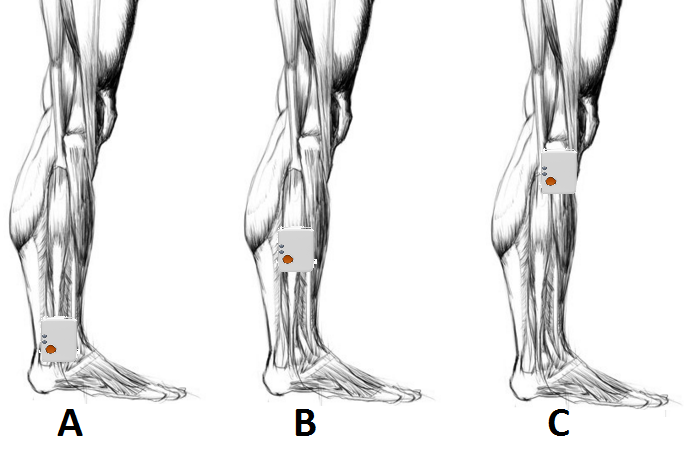
\includegraphics[scale=0.6]{figures/qBilag/Sensor_placering2.png}
	\caption{På figuren ses, hvor sensoren skal placeres under pilotforsøget. Placering A viser sensoren siddende proximalt over den laterale malleolus. Placering B illustrerer sensoren, når den er medialt på den ventrale side af tibia. I placering C er sensoren distalt for patella. \textbf{HUSK AT TEKSTEN SKAL PASSE TIL DET NYE BILLEDE} (Modificeret fra \cite{Perna2016,Shimmer2016})}
	\label{fig:sensor_placering}
\end{figure}


Første måling involverer aktiviteten, gang. Førend målingen udføres skal forsøgspersonen besvære hvilket trin som denne befinder sig på i forhold til Borgskalaen. Herefter startes løbebåndet og indstilles til en hastighed på 4,8 km/t. Forsøgspersonen går på løbebåndet mens hastigheden stiger, således der er en homogen bevægelses-cyklus ved en givne hastighed. Forsøgspersonen indikerer når denne føler en homogen bevægelses-cyklus. Derefter påbegyndes målingen og har en varighed på 45 sekunder. 

Næste aktivitet involverer løb, hvortil hastigheden er 11,3 km/t. Forsøgspersonen besvarer hvilket trin denne befinder sig på i forhold til Borgskalaen. Efterfølgende skal forsøgspersonen opnå en homogen bevægelses-cyklus mens hastigheden stiger op til den indstillede hastighed. Forsøgspersonen indikerer når der er en homogen bevægelses-cyklus, hvorefter målingen foretages i 45 sekunder. 

Der skal ligeledes foretages en måling, hvor hastigheden på løbebåndet gradvist øges fra 0 km/t indtil forsøgspersonen ikke kan løbe hurtigere. Forsøgspersonen besvarer hvilket trin denne befinder sig på i forhold til Borgskalaen, inden forsøget påbegyndes. \newline
Forsøget starter med en stillestående forsøgsperson på løbebåndet, hvorefter løbebåndes startes og indstilles til en hastighed på 2 km/t som varer i 20 sekunder. Herefter stiger hastigheden gradvist med 2 km/t hver gang forsøgspersonen har bevæget sig i 20 sekunder. Når forsøgspersonen har opnået sin maksimale hastighed, eller løbebåndets maksimale hastighed, da stoppes målingen. Undervejs noteres det endvidere hvornår forsøgspersonen skifter fra gang til løb. 

Sidste måling foregår på en motionscykel, hvor forsøgspersonen først besvarer hvilket trin denne befinder sig på i forhold til Borgskalaen. Efterfølgende skal forsøgspersonen opnå en homogen bevægelses-cyklus med en hastighed på 20,9 km/t ved en belastning på 35 W. Når forsøgspersonen indikerer at der er tale om en homogen bevægelses-cyklus, da påbegyndes målingen på 45 sekunder. 


\section{Databehandling}

\section{Resultater}

\section{Diskussion}

\section{Konklusion}

%% Opgaver - rettelser
% Man skal markere på forsøgspersonen med tush eller andet hvor sensoren skal placeres